\documentclass{ltjsarticle}

\usepackage{graphics}
\begin{document}

\title{LilyPond-Bookによる楽典資料生成試験}
\author{haru}
\maketitle

\tableofcontents
\clearpage

\section{音符の種類}

音符にはその長さ(「音価」という)によって複数の種類が存在する。\\

{%
\parindent 0pt
\noindent
\ifx\preLilyPondExample \undefined
\else
  \expandafter\preLilyPondExample
\fi
\def\lilypondbook{}%
\includegraphics{/mnt/c/Users/haru/working/zenn-test-2/test/bc/lily-5f895ac8-1}%
% eof
%
\ifx\postLilyPondExample \undefined
\else
  \expandafter\postLilyPondExample
\fi
}

上記の譜面は、譜面上の「ソ」の位置に音符をプロットした例である。 \\
左から順に、全音符、二分音符、四分音符、八分音符、十六分音符、三十二分音符である。

\section{調}

音楽の雰囲気を決定づけるものとして、最も重要なのは「調」である。\\
この「調」は「長調」と「短調」に分けられ、それぞれに12種類ずつ存在する。

\subsection{長調}

一般に明るいイメージを抱かれる。\\
ここでは代表的な長調として「ハ長調」(C-dur, C Major)を示す。

{%
\parindent 0pt
\noindent
\ifx\preLilyPondExample \undefined
\else
  \expandafter\preLilyPondExample
\fi
\def\lilypondbook{}%
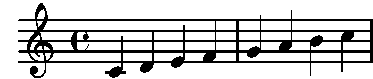
\includegraphics{/mnt/c/Users/haru/working/zenn-test-2/test/e0/lily-29933f20-1}%
% eof
%
\ifx\postLilyPondExample \undefined
\else
  \expandafter\postLilyPondExample
\fi
}

なお、他の調においても構成音の間隔は変化しない。

{%
\parindent 0pt
\noindent
\ifx\preLilyPondExample \undefined
\else
  \expandafter\preLilyPondExample
\fi
\def\lilypondbook{}%
\includegraphics{/mnt/c/Users/haru/working/zenn-test-2/test/f1/lily-294e6d57-1}%
% eof
%
\ifx\postLilyPondExample \undefined
\else
  \expandafter\postLilyPondExample
\fi
}

上に示したのはヘ長調(F-dur, F Major)である。

\end{document}
